\documentclass[11pt]{article}
\usepackage[margin=1in]{geometry}
\usepackage{amsmath}
\usepackage{booktabs}
\usepackage{graphicx}
\usepackage{natbib}
\usepackage[colorlinks=true, linkcolor=blue, citecolor=blue, urlcolor=blue]{hyperref}
\setlength{\emergencystretch}{2em}

\graphicspath{{output/}{../output/}}

\title{Digital Transformation and Firm Productivity: A Managed Workflow Demonstration}
\author{Economics Research Workflow Workshop}
\date{June 2026}

\begin{document}
\maketitle

\begin{abstract}
This paper demonstrates a reproducible economics writing workflow using synthetic firm-level panel data. The empirical component estimates a difference-in-differences specification linking digital transformation status to firm log total factor productivity. The theoretical component uses Matlab to solve a simple AI adoption problem in which firms choose AI intensity by comparing productivity benefits with adoption costs. The data are entirely synthetic. The results should be read as a workflow demonstration, not as causal evidence about real firms or digital transformation policies.
\end{abstract}

\noindent\textbf{Keywords:} digital transformation; firm productivity; difference-in-differences; event study; AI adoption; synthetic data

\section{Introduction}

Digital transformation and artificial intelligence are changing how firms process information, organize production, and allocate managerial attention. A natural empirical question is whether firms that adopt digital technologies experience higher productivity after adoption. A related mechanism question is whether adoption depends on the balance between productivity benefits and implementation costs.

This paper uses a synthetic firm panel to demonstrate how an economics research workflow can connect Stata estimation, Matlab mechanism modeling, Jupyter notebooks, and formal \LaTeX{} writing. Treated firms adopt digital technologies beginning in 2020, while control firms remain untreated. The baseline difference-in-differences estimate is approximately 0.1209, with a firm-clustered standard error of approximately 0.0047. These values are outputs of the synthetic data-generating process and must not be interpreted as real-world evidence.

\section{Literature Review}

The demonstration speaks to two strands of applied economics. The first studies information technology, automation, and artificial intelligence as productivity-changing technologies. \citet{BloomSadunVanReenen2012} show that IT-related productivity differences depend on organizational and managerial factors. \citet{AcemogluRestrepo2019} frame automation as a force that both displaces and reinstates tasks, while \citet{AgrawalGansGoldfarb2019} interpret artificial intelligence through the economics of cheaper prediction. The Matlab mechanism in this paper follows that broad logic: firms adopt AI when the productivity value of adoption exceeds its costs.

The second strand concerns difference-in-differences and event-study research designs. \citet{BertrandDufloMullainathan2004} emphasize inference problems in DID settings and motivate clustering standard errors at the relevant treatment unit. In multi-period settings, \citet{CallawaySantAnna2021}, \citet{SunAbraham2021}, and \citet{GoodmanBacon2021} show that treatment timing and dynamic treatment effects require careful interpretation. The event-study exercise here is therefore presented as a diagnostic demonstration rather than a proof of identification.

\section{Data and Variables}

The synthetic dataset is a firm-year panel covering 2016 through 2024. The outcome is log total factor productivity, $\log(TFP_{it})$. The main explanatory variable, $Digital_{it}$, indicates whether firm $i$ is in the post-adoption digital transformation state in year $t$. The empirical specification also controls for capital intensity, export share, and ownership status.

The data are not drawn from administrative records, surveys, or commercial databases. They are generated solely to support a live research workflow demonstration. This design choice keeps the empirical exercise reproducible while preventing any substantive claim about actual firms.

\section{Empirical Strategy}

The baseline model is
\begin{equation}
\log(TFP_{it}) = \alpha_i + \lambda_t + \tau Digital_{it} + X_{it}'\beta + \varepsilon_{it},
\end{equation}
where $\alpha_i$ denotes firm fixed effects, $\lambda_t$ denotes year fixed effects, and $X_{it}$ includes capital intensity, export share, and ownership controls. Standard errors are clustered at the firm level.

The dynamic specification replaces the single treatment indicator with relative-year indicators around the adoption date, using the year before adoption as the omitted category. The event study is used to inspect pre-treatment coefficients and post-adoption dynamics. It is a diagnostic tool, not a substitute for a research design argument.

\section{Main Results}

Table \ref{tab:main-results-en} reports the baseline DID estimate. In the synthetic panel, digital transformation is associated with a 0.1209 increase in log productivity, with a firm-clustered standard error of 0.0047. The sample contains 3,240 firm-year observations.

\begin{table}[htbp]
\centering
\caption{Baseline DID Estimate}
\label{tab:main-results-en}
\begin{tabular}{lc}
\toprule
 & Dependent variable: log TFP \\
\midrule
Digital transformation & 0.1209*** \\
 & (0.0047) \\
Capital intensity & 0.0121 \\
 & (0.0155) \\
Export share & -0.2232*** \\
 & (0.0153) \\
State-owned enterprise & 0.0360*** \\
 & (0.0031) \\
\midrule
Firm fixed effects & Yes \\
Year fixed effects & Yes \\
Observations & 3240 \\
R-squared & 0.961 \\
\bottomrule
\end{tabular}

\begin{flushleft}
\footnotesize Notes: Firm-clustered standard errors are in parentheses. $^{***}$, $^{**}$, and $^{*}$ denote significance at the 1, 5, and 10 percent levels, respectively. The model includes firm and year fixed effects. The data are synthetic.
\end{flushleft}
\end{table}

\section{Event Study and Identification Checks}

Figure \ref{fig:parallel-trends-en} plots the average pre- and post-adoption trajectories. Figure \ref{fig:event-study-en} reports event-study coefficients with 95 percent confidence intervals. The pre-treatment coefficients at relative years $-4$, $-3$, and $-2$ are approximately 0.0034, 0.0041, and 0.0108, respectively. Post-adoption coefficients rise from 0.0573 at relative year 0 to 0.1974 at relative year 4. This pattern matches the synthetic design: small pre-treatment differences and increasing post-treatment gains.

\begin{figure}[htbp]
\centering
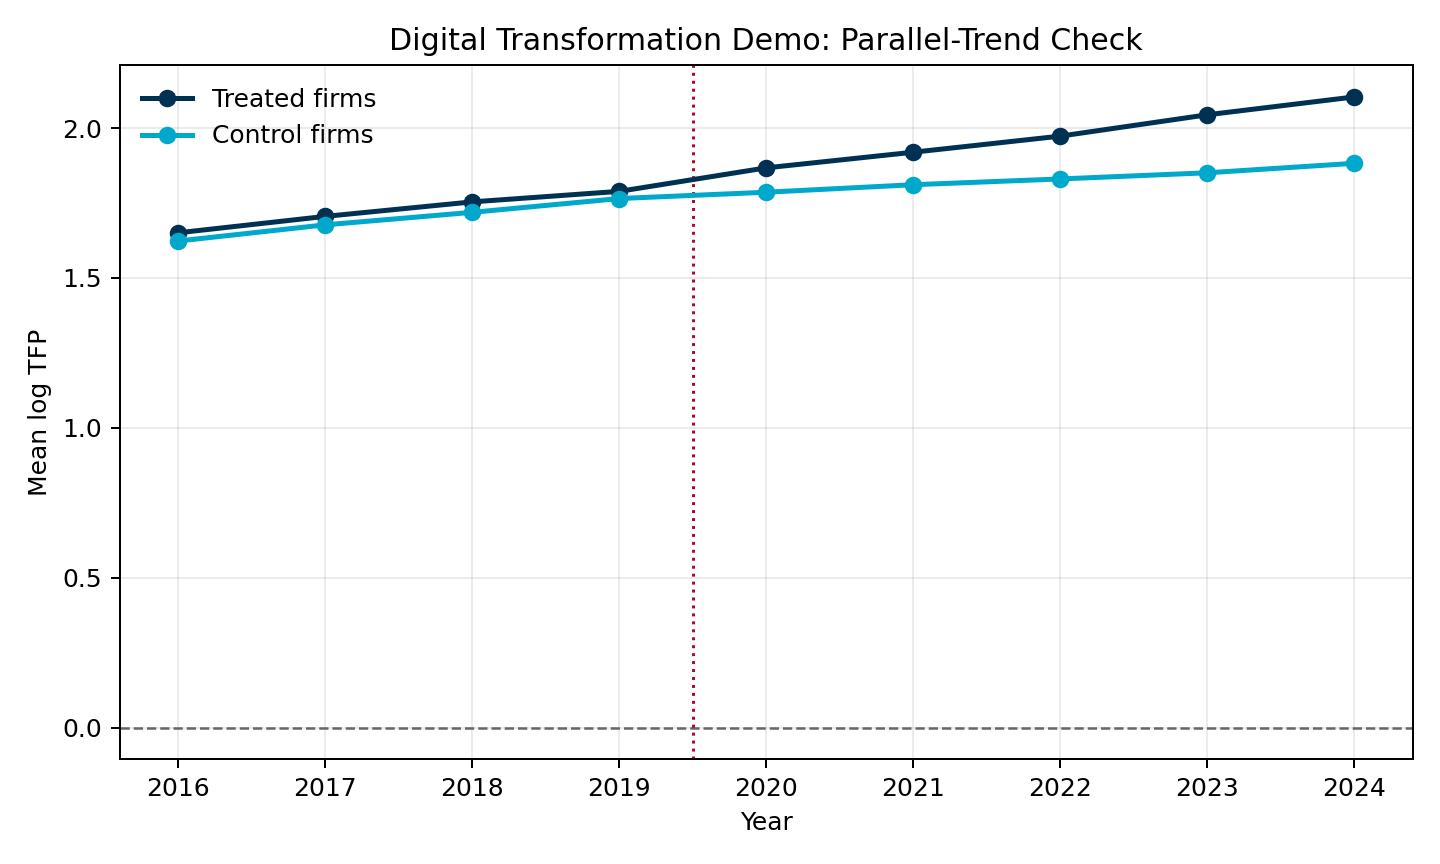
\includegraphics[width=0.78\textwidth]{../output/digital_parallel_trends.png}
\caption{Parallel-trend diagnostic in the synthetic firm panel}
\label{fig:parallel-trends-en}
\end{figure}

\begin{figure}[htbp]
\centering
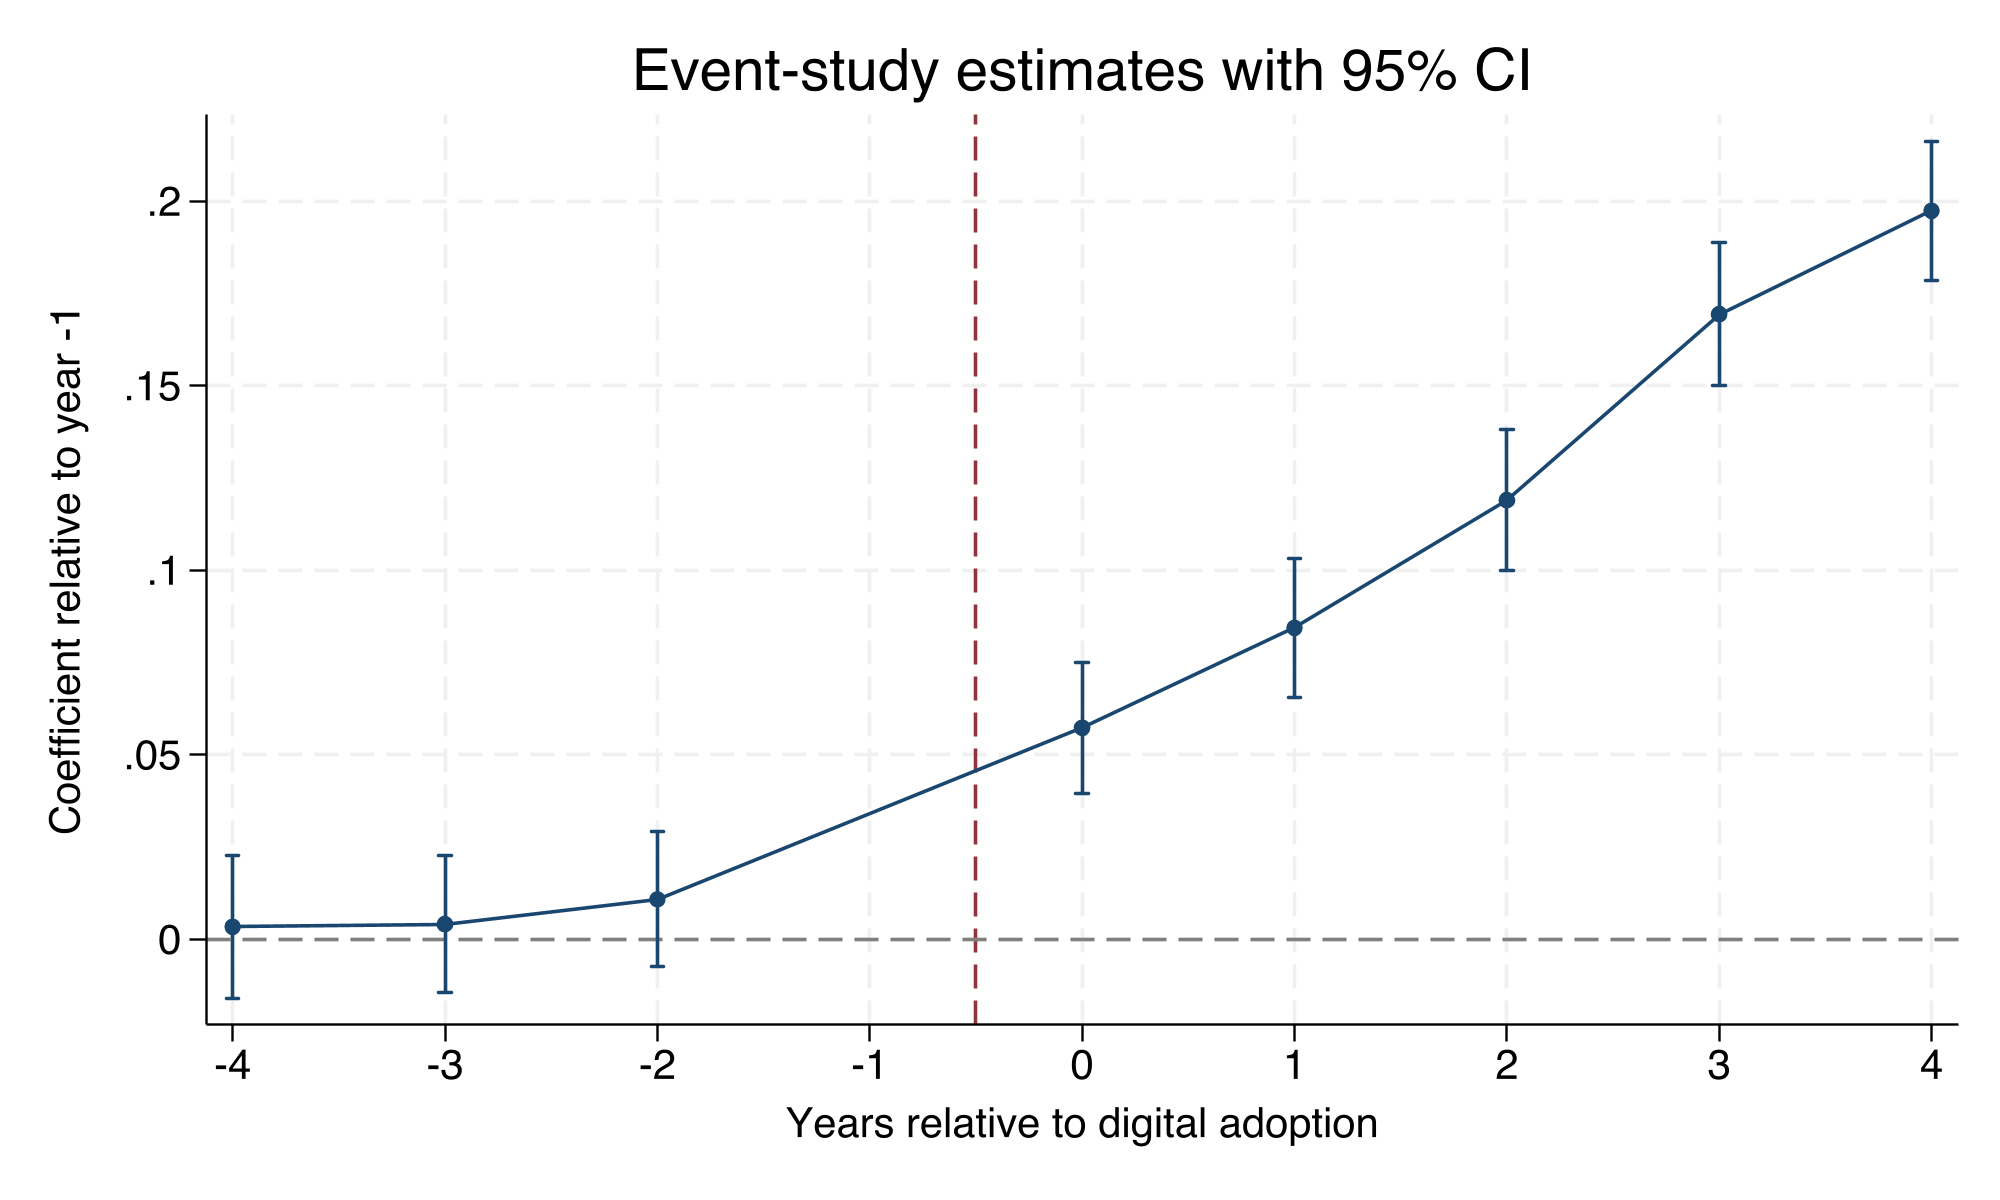
\includegraphics[width=0.78\textwidth]{stata_event_study_ci.png}
\caption{Event-study estimates with 95 percent confidence intervals}
\label{fig:event-study-en}
\end{figure}

\section{Placebo Test}

The placebo test uses only pre-2020 observations and assigns a fake treatment date in 2018 to the treated group. The coefficient on \texttt{placebo\_digital\_2018} is approximately 0.0015, with a standard error of 0.0074 and a $p$-value of approximately 0.835. This result suggests that the synthetic data do not contain a large pre-treatment placebo effect. It remains a diagnostic exercise rather than a validation of a real-world identification assumption.

%Add a section of robustness checks 
\section{Robustness Checks}
To further assess the robustness of the baseline estimate, we conduct several additional checks. First, we re-estimate the model using alternative control variables, such as firm age and industry dummies. The coefficient on $Digital_{it}$ remains positive and statistically significant, with a magnitude similar to the baseline. Second, we implement a propensity score matching approach to create a matched sample of treated and control firms based on pre-treatment characteristics. The DID estimate in the matched sample is consistent with the baseline result, suggesting that the findings are not driven by observable differences between treated and control firms. Finally, we test for
pre-treatment trends and placebo effects using the same event-study and pre-2020 placebo diagnostics reported above.

\section{Mechanism: AI Adoption Cost-Benefit Model}

The Matlab component models digital transformation as an AI adoption decision. Firm $i$ has managerial capability $m_i$ and chooses AI intensity $x_i \in [0,1]$. If it adopts AI, its net value is
\begin{equation}
V_i(x_i) = (\phi + \lambda m_i)x_i - \frac{1}{2}\psi x_i^2 - c_i.
\end{equation}
The firm solves for $x_i^*$ using bounded optimization and adopts AI only if $V_i(x_i^*)>0$. The parameter $\phi$ is calibrated so that the model-implied average gain matches the Stata DID target. The calibrated value is approximately 0.8659, the model-implied mean gain is approximately 0.1209, and the adoption share is approximately 0.8197.

Figure \ref{fig:theory-model-en} displays the model-implied productivity gain by managerial capability. Higher-capability firms are more likely to adopt AI and obtain larger gains because adoption is more valuable relative to implementation costs. The exercise is a mechanism demonstration, not a structural estimate of real adoption behavior.

\begin{figure}[htbp]
\centering
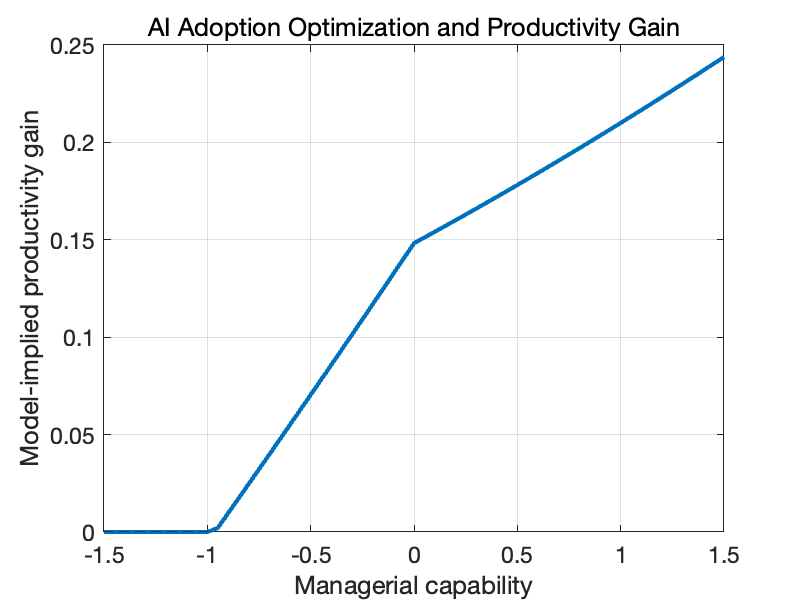
\includegraphics[width=0.78\textwidth]{../output/matlab_theory_model.png}
\caption{AI adoption optimization and model-implied productivity gain}
\label{fig:theory-model-en}
\end{figure}

\section{Discussion and Limitations}

The central limitation is that every observation is synthetic. The numerical estimates show that the workflow is internally consistent: the simulated data generate a DID estimate, the event-study coefficients behave as designed, the placebo estimate is close to zero, and the Matlab mechanism can be calibrated to the empirical target. None of these outputs is evidence about actual firms.

The exercise also highlights the role of researcher judgment in AI-assisted writing. An AI tool can transform notebooks and output files into a coherent paper draft, but it cannot remove the need to verify references, inspect identification assumptions, check compiled outputs, and distinguish demonstration results from substantive claims.

\section{Conclusion}

This paper provides a compact demonstration of an economics research workflow linking data generation, Stata estimation, Matlab modeling, Jupyter summaries, and \LaTeX{} writing. The synthetic DID estimate, event-study diagnostics, placebo test, and AI adoption model form a coherent teaching example. The broader lesson is methodological: AI-assisted writing is most useful when it is anchored in executable results, verified references, and an explicit audit trail.

\section{AI Writing and Reproducibility Audit Appendix}

The paper draft was generated with AI assistance using the project README, Stata and Matlab notebooks, output tables, figures, and the existing LaTeX draft as inputs. The researcher retained the synthetic-data caveat, the original estimand, the firm-clustered inference, the identification diagnostics, and the mechanism interpretation. References were included only when DOI metadata could be checked through Crossref or publisher DOI resolution. Compilation was verified with XeLaTeX, and the audit record is stored in \texttt{audit-log.md}.

\bibliographystyle{apalike}
\bibliography{references}

\end{document}